% =====================================================================
%  2026-05-11 — 第二次去光華:用 MUX 把波段開關吃掉的關鍵 insight
% =====================================================================

\subsection*{今日目標}

\begin{itemize}[leftmargin=2em,itemsep=0pt]
  \item 回光華補 4/21 漏買的東西 \texttt{+} 解掉 5/6 麵包板實驗暴露出來的兩個痛點。
  \item 順路取 5/7 下單的 \textbf{Fnirsi HS-02A} 烙鐵(取件 13:25)。
  \item 把 5/3 那張「四檔旋鈕」的設計圖再升級一階:用 MCU 控制的類比 mux 取代純機械的波段開關。
\end{itemize}

\subsection*{關鍵 insight:用 ADC 動態範圍當「自動切檔」訊號}

5/6 量測復盤的時候發現一件事:Pico ADC 雖然名義上吃 0--3.3 V,但兩端各有一塊 dead zone:

\begin{itemize}[leftmargin=2em,itemsep=0pt]
  \item 下限:5/6 在 TIA 的 \(+\) 端故意墊了 \(V_\text{ref} \approx \SI{0.1}{\volt}\),
        所以 \(V_\text{OUT}\) 永遠 \(\gtrsim 0.1\) V;再加 op-amp 接近 0 V 的非線性,
        實際可用下限 \(\approx \SI{0.3}{\volt}\)。
  \item 上限:rail-to-rail 雖然能到 3.3 V,但接近上軌也有非線性 + clipping;
        實際可用上限 \(\approx \SI{3.0}{\volt}\)。
\end{itemize}

也就是「線性可用區」其實只有 \(\sim \SI{0.3}{\volt}\)--\(\SI{3.0}{\volt}\) 這一段。
原本以為兩端 dead zone 是浪費,但反過來看:它們其實是\textbf{現成的「該換檔了」訊號}。

\begin{itemize}[leftmargin=2em,itemsep=0pt]
  \item \(V_\text{OUT} \to \SI{3.0}{\volt}\) \(\Rightarrow\) 飽和了 \(\Rightarrow\) 該往\textbf{低增益}檔切。
  \item \(V_\text{OUT} \to \SI{0.3}{\volt}\) \(\Rightarrow\) 底噪了 \(\Rightarrow\) 該往\textbf{高增益}檔切。
  \item \(V_\text{OUT}\) 落在 \(0.3\)--\(3.0\) 中間 \(\Rightarrow\) 維持當前檔。
\end{itemize}

只要把 Pico 程式裡塞個 hysteresis-based 自動換檔狀態機,就能讓 flico
\textbf{不用人手動轉旋鈕}就在四檔之間無縫滑動。這是「智慧 flico」的第一個雛形。

\subsection*{硬體實作:74HC4051 取代機械式波段開關}

要讓 Pico GPIO 能切換 \(R_F\) 路徑,需要一顆\textbf{類比多工器 (analog multiplexer)}:

\begin{itemize}[leftmargin=2em,itemsep=0pt]
  \item 元件:\textbf{74HC4051}(8 通道單刀類比 mux,但這裡只用 4 通道對應四檔)。
  \item 接法:把 \texttt{COM} 接到 op-amp 的反相輸入,\texttt{Y0--Y3} 各接一顆 \(R_F\)
        (1 k / 10 k / 100 k / 1 M),另一端統一接 \(V_\text{OUT}\)。
        Pico GPIO 控 \texttt{S0/S1}(\texttt{S2} 拉地)做四選一。
  \item 4/19 跟 Gemini 討論時就提過 TMUX1104 這條路,當時覺得太進階,
        今天決定直接走 mux。74HC4051 在光華有貨、便宜、DIP 封裝可插麵包板,門檻最低。
  \item 雖然採購了一顆\textbf{傳統 1P4T 波段開關備援}(50 元),先當 fallback;
        若 mux 自動換檔搞不出來,還可以手動切。
\end{itemize}

\subsection*{順手解掉 5/6 留下的兩個痛點}

\begin{enumerate}[leftmargin=2em,itemsep=2pt]
  \item \textbf{杜邦線太亂、BPW34 翹起來貼不到螢幕} \(\to\) 買了 \textbf{140 根預剪硬跳線盒}。
        硬跳線可以走平貼麵包板的水平路徑,BPW34 就能乖乖貼螢幕了。
  \item \textbf{每換一檔 \(R_F\) 都要拔線} \(\to\) 上面的 74HC4051 mux 直接幹掉這件事,
        而且還順便升級成「MCU 自動切」(原本只是想要旋鈕)。
\end{enumerate}

\subsection*{今天另一條線:第一次接 OLED 用 I\textsuperscript{2}C 跑 SSD1306}

5/8 那天本來打算順手把 OLED 也接上,但當時沒貨;今天買到自己的 \textbf{0.91" SSD1306 OLED} 就把這條線補完,
flico 第一次有了「Pico 自己也會講話的螢幕」。

\begin{itemize}[leftmargin=2em,itemsep=0pt]
  \item \textbf{接腳}:I\textsuperscript{2}C0,\texttt{SDA=GP4 / SCL=GP5};
        OLED 預設 7-bit 地址 \texttt{0x3C}、解析度 \(128 \times 32\)。
  \item \textbf{驅動}:從 0 寫了 \texttt{ssd1306.py},繼承 MicroPython 內建的 \texttt{framebuf.FrameBuffer};
        提供兩個 class:
        \begin{itemize}[leftmargin=2em,itemsep=0pt]
          \item \texttt{SSD1306} —— 底層 \texttt{init\_display()} 寫 OLED 控制字
                (set MUX ratio / segment remap / charge pump 等十幾個命令),
                以及 \texttt{show()} 把 framebuf 推進顯示記憶體。
          \item \texttt{SSD1306\_I2C(SSD1306)} —— I\textsuperscript{2}C 包裝層,
                \texttt{write\_cmd} 走控制 byte \texttt{0x80}、
                \texttt{write\_data} 用 \texttt{writevto} 一次推 framebuf 整塊。
        \end{itemize}
  \item \textbf{整合到 main.py}:
        \texttt{oled.fill(0)} \(\to\) \texttt{oled.text("V=...", 0, 0)} \(\to\) \texttt{oled.show()}
        三步把瞬間電壓秀到螢幕。同樣的 ADC 讀取迴圈,5/8 還只是 print 到 console,
        今天\textbf{連電腦都不用接也能看讀數}。
  \item 對應檔:\texttt{firmware/python-version/ssd1306.py}(99 行,大半是 SSD1306 啟動序列那一段)。
\end{itemize}

把這條線打通的瞬間,5/3 提案書畫的「裝置正面」配置(感光窗 + 4 位 7 段顯示器 + 旋鈕 + 模式開關)
開始跟現實對得起來 —— 雖然今天用的是 OLED 不是 7 段,但 \textbf{flico 已經是一台「站著也能用」的儀器了},
不再是麵包板加一條杜邦線到三用電表那種「躺著實驗」階段。

\subsection*{購買清單與收據}

12:51 結帳於\textbf{今華電子}(同 4/21 那家),刷掉 \(\textbf{TWD 735}\) 現金、找回 65 元
(付 800)。收據如圖~\ref{fig:0511-receipt}。

\begin{figure}[H]
  \centering
  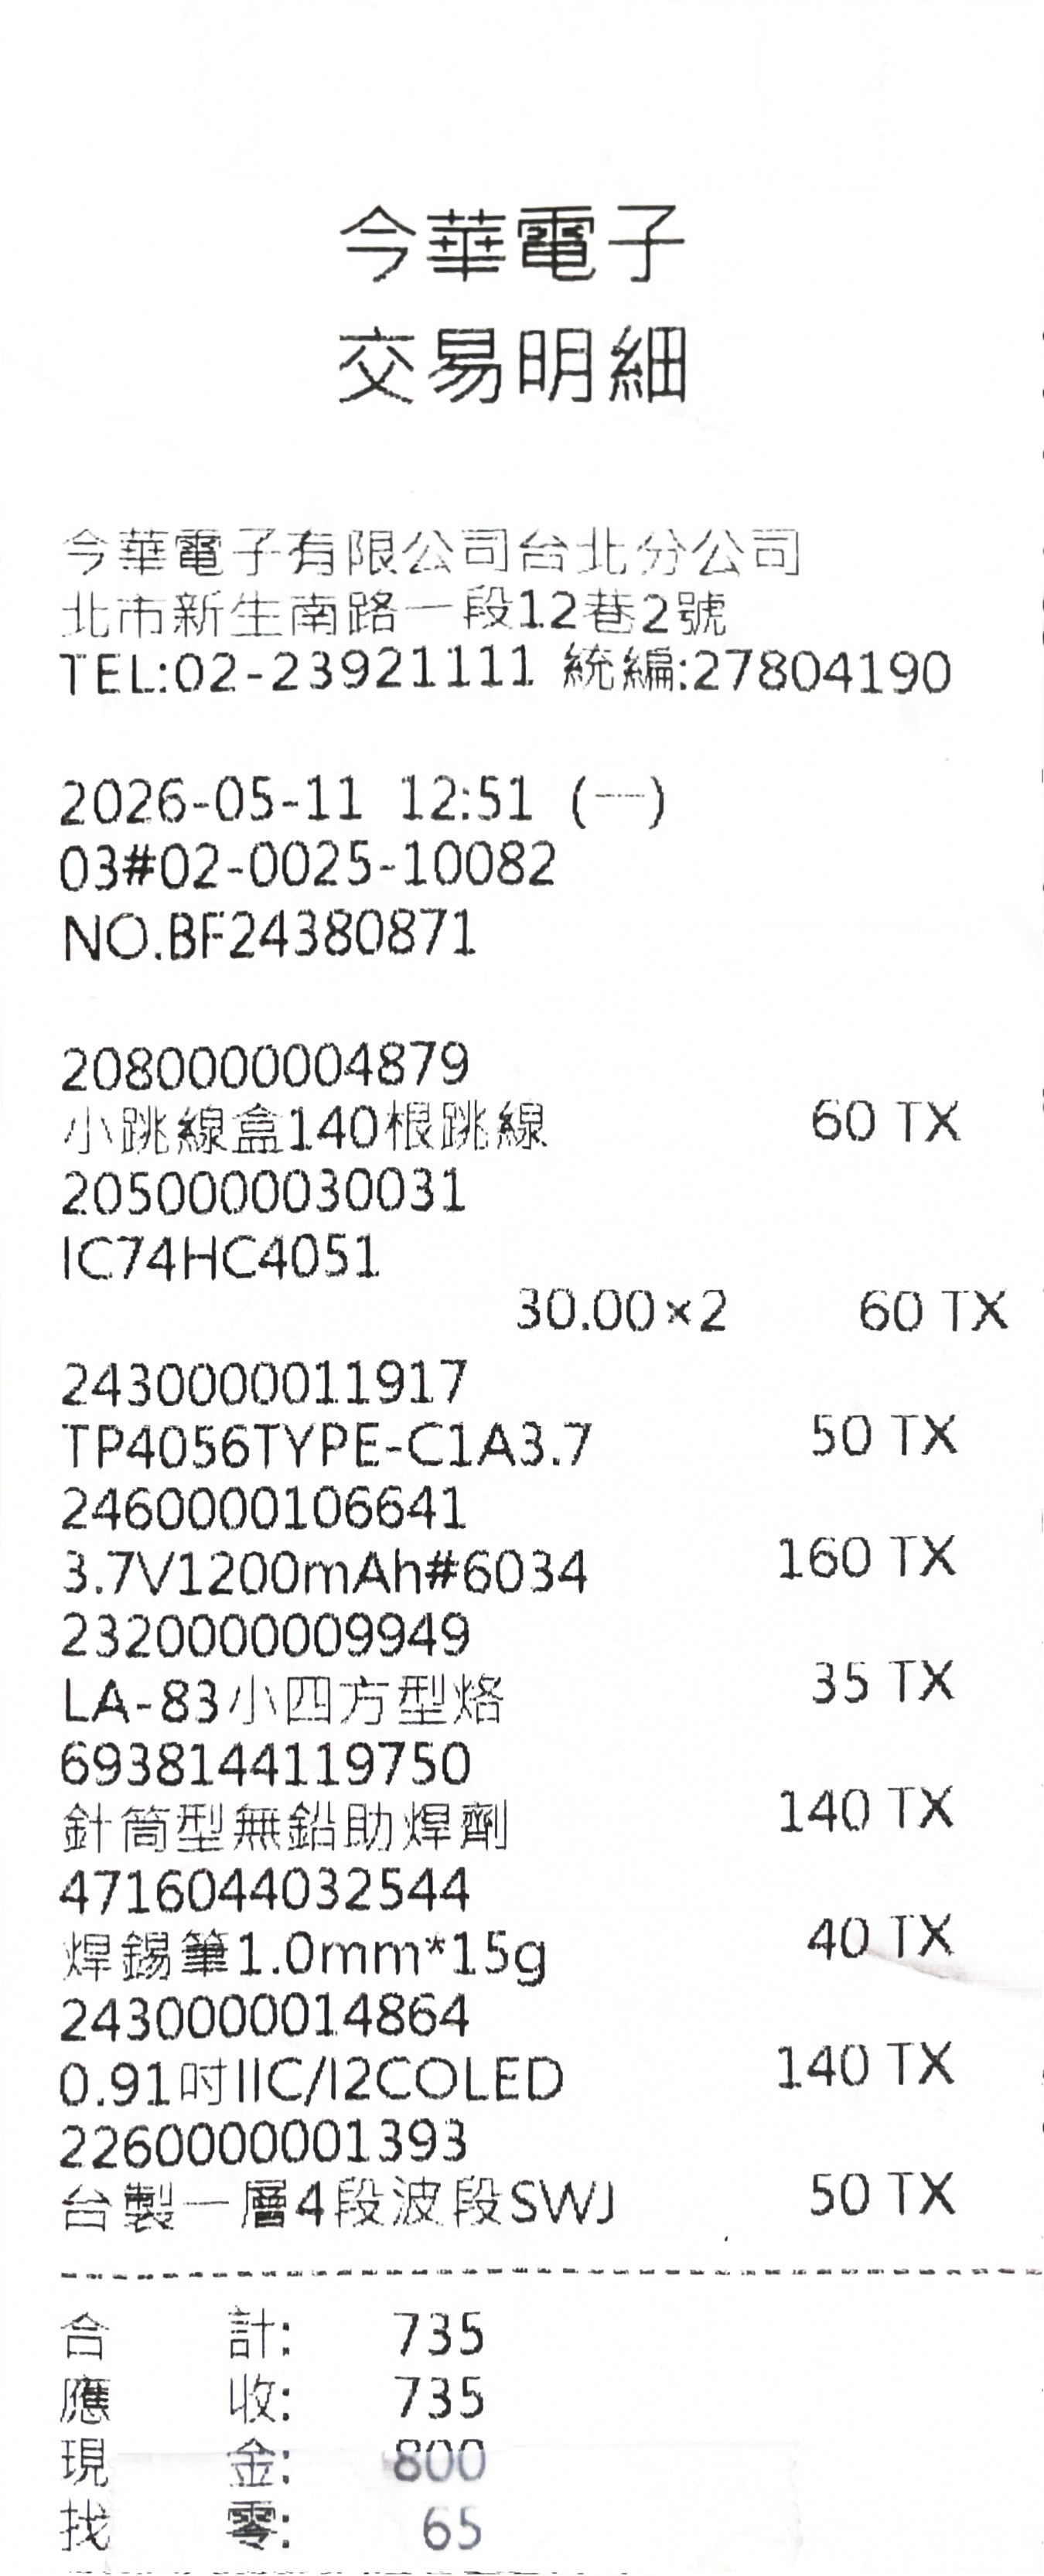
\includegraphics[width=0.55\linewidth]{2026-05-11/今華電子交易明細0511.jpg}
  \caption{今華電子 2026-05-11 12:51 第二次交易明細,合計 TWD 735。}
  \label{fig:0511-receipt}
\end{figure}

\begin{table}[H]
  \centering
  \caption{5/11 今華電子採購明細。}
  \label{tab:0511-bom}
  \begin{tabular}{llrr}
    \toprule
    類別 & 品項 & 數量 & 小計 (TWD) \\
    \midrule
    接線     & 小跳線盒 140 根預剪跳線              & 1 & 60  \\
    增益切換 & 74HC4051 8 通道類比 MUX(DIP-16)     & 2 & 60  \\
    增益切換 & 台製 1 層 4 段波段開關(備援)         & 1 & 50  \\
    電源     & TP4056 Type-C 1A 鋰電池充電板         & 1 & 50  \\
    電源     & 3.7 V / 1200 mAh LiPo 電池(\#6034)    & 1 & 160 \\
    顯示     & 0.91" I\textsuperscript{2}C SSD1306 OLED & 1 & 140 \\
    焊接     & LA-83 小四方形烙鐵架(海綿底座)        & 1 & 35  \\
    焊接     & 針筒型無鉛助焊劑(松香膏)              & 1 & 140 \\
    焊接     & 焊錫筆 1.0 mm \texttimes{} 15 g       & 1 & 40  \\
    \midrule
    \multicolumn{3}{r}{\textbf{合計(付現)}} & \textbf{735} \\
    \multicolumn{3}{r}{\textbf{付 800,找 65}} & \\
    \bottomrule
  \end{tabular}
\end{table}

幾個現場決定的細節:

\begin{itemize}[leftmargin=2em,itemsep=0pt]
  \item \textbf{74HC4051 ×2}:第二顆是備援,寒流發抖手抖燒一顆便宜很多。
  \item \textbf{TP4056 加上 LiPo 一起買}:5/3 提案書時候就決定電源走「3.7 V LiPo \(\to\) LDO \(\to\) 3.3 V」,
        今天把上游一次備齊;LDO 之前光華沒貨,留作下次。
  \item \textbf{0.91" OLED}:5/8 本來想接 OLED 但根本沒貨,今天先把感測器買回家,
        當天稍晚才正式接上去跑(詳上節「今天另一條線」)。
  \item \textbf{LA-83 烙鐵架 + 助焊劑 + 焊錫}:都是 5/7 下單烙鐵的配套耗材,
        準備今天 13:25 取件回家就直接焊。
\end{itemize}

回家拆袋順手拍了 LiPo 電池實物,做個檔案備存(圖~\ref{fig:0511-lipo});
注意黃色絕緣膠帶下面就是保護板,使用前要確認 TP4056 模組的 B\(+\)/B\(-\) 不能跟電池正負極接反。

\begin{figure}[H]
  \centering
  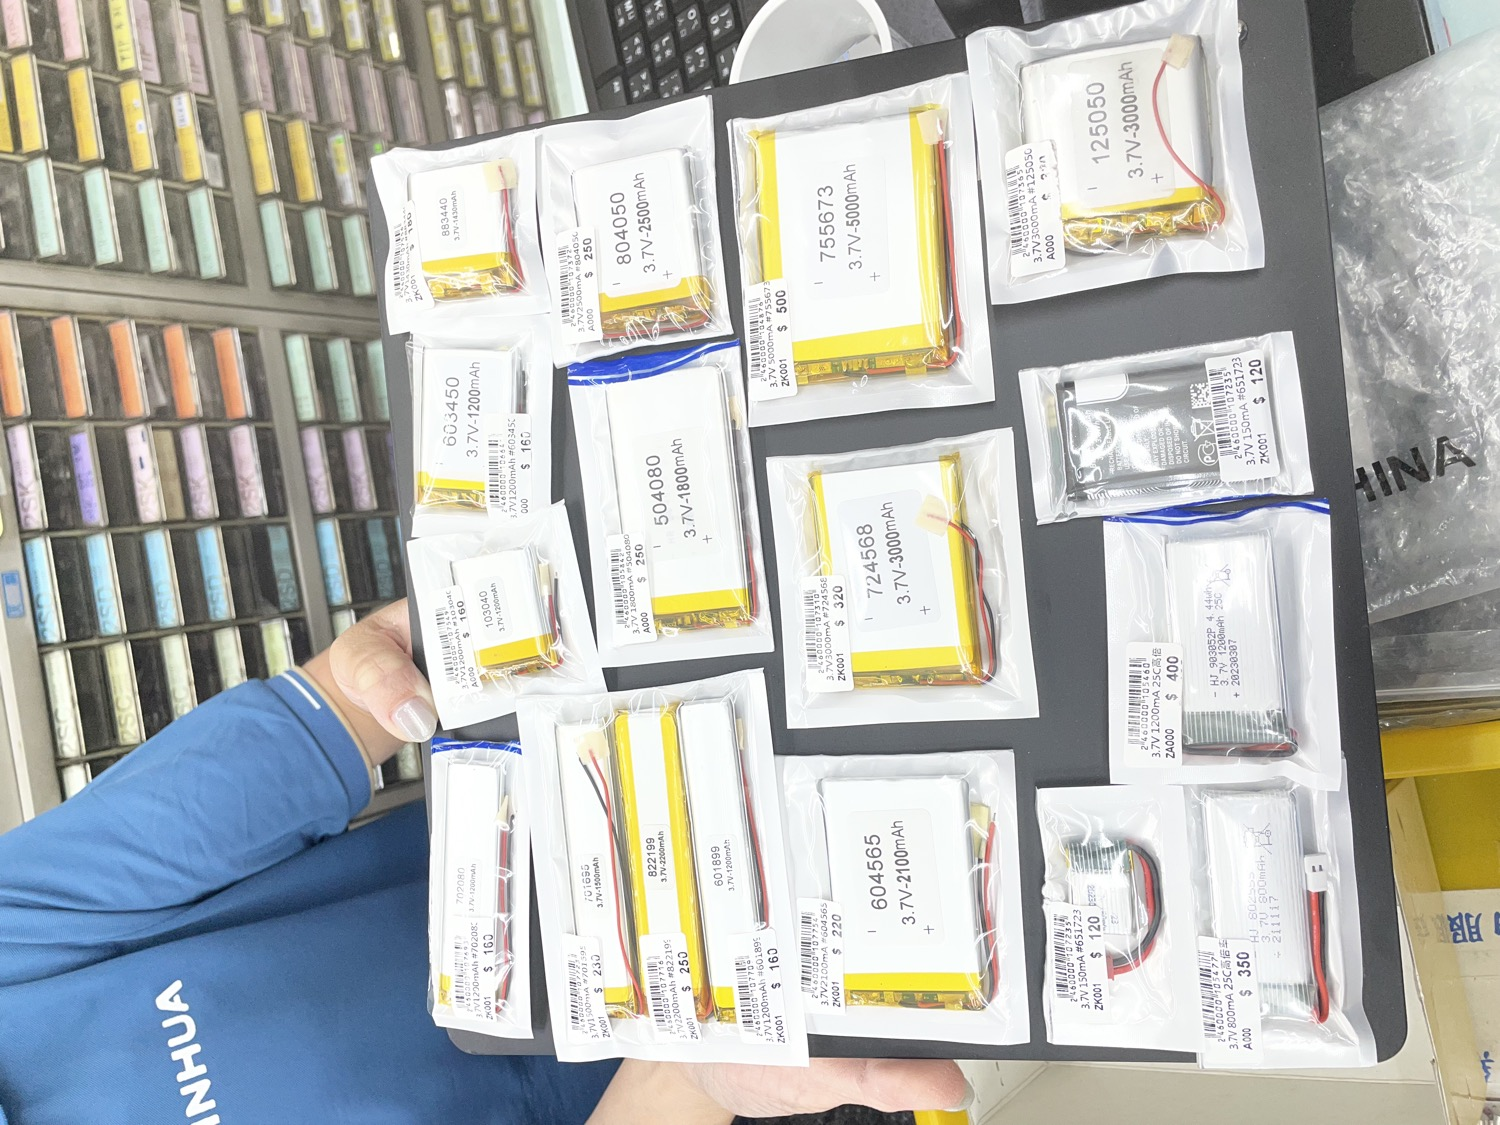
\includegraphics[width=0.55\linewidth]{2026-05-11/LiPo.jpg}
  \caption{今天買到的 3.7 V / 1200 mAh LiPo 電池(\#6034),
           回家拆袋後拍下實物存檔;原始 HEIC 留在
           \texttt{figures/2026-05-11/LiPo.HEIC}。}
  \label{fig:0511-lipo}
\end{figure}

\subsection*{今日心得}

\begin{itemize}[leftmargin=2em,itemsep=0pt]
  \item \textbf{今天最大的突破不是買到任何零件,而是發現 ADC 兩端的「dead zone」可以當訊號用}。
        原本以為要犧牲 \(\sim 18\%\) 的動態範圍,
        現在反過來看 \(\Rightarrow\) 那 18\% 就是免費的「該換檔」自動訊號。
        一個 \texttt{if v > 3.0: switch\_to\_lower\_gain()} 的迴圈,
        加 hysteresis 防抖,系統就比手轉旋鈕還聰明。
  \item \textbf{硬體界線一直在動}:4/19 時想用機械旋鈕,
        4/21 想著買波段開關沒買到,今天直接跳級到 mux + MCU 控制。
        每次重新想都比上次省一點手動操作,這就是迭代設計該有的方向。
  \item 0.3 V 跟 3.0 V 這兩個門檻數字得校準,有溫漂跟個體差,
        \textbf{下一步}:接上 74HC4051 量四檔的實際飽和點 + 底噪點,
        作為自動換檔狀態機的常數;同時下單 LDO(HT7133 或 XC6206-3.3V)
        把電池供電鏈補齊。
\end{itemize}
